%
% Draft  document crimptype.tex
% Classifying sheep as (stretched,unaligned,unfolded) based on visual wool scores done on-sheep
%
 
\documentclass[titlepage]{article}  % Latex2e
\usepackage{graphicx,lscape,subfigure}
\usepackage{bm}
\usepackage{textcomp}
\usepackage[flushleft]{threeparttable}
 

\title{Classifying sheep into crimp types using on-sheep visual wool scores and measures. Part I Original crimp type assessment and Zigzag visual crimp scores. }
\author{Jim Watts and Neville Jackson}
\date{7 Feb 2017} 

 
\begin{document} 
 
\maketitle      
\tableofcontents

\clearpage
\section{Introduction} 
It has been shown that crimp forms in a Merino wool staple in two geometrically different ways, termed {\em stretched helix} and {\em unfolded helix} by Jackson and Watts(2016)~\cite{jack:16}.  These two forms of crimp can not be visually recognised, except in extreme cases. A {\em stretched helix} crimp is 3-dimensional and looks like a sine wave in planar view. An {\em unfolded helix} crimp is 2-dimensional and looks like a semicircular wave, which in extreme cases has a {\em horseshoe} appearance. Without magnification, classing wools into these two crimp types is difficult.
 
There is therefore interest in seeing whether one can classify wools into these two crimp type classes, using an armoury of scores and measurements which can be conducted on the sheep. The logic is that the two crimp types will either cause or be correlated with a number of other observable staple properties. Here we use 4 measurements and six scores.

We actually make 3 crimp types. The {\em stretched helix} type is subdivided into {\em unaligned} which has poor fibre alignment to that the staple crimp is obscured by a {\em haze} of fibres not in phase with the crimp wave, and {\em stretched} which has good fibre alignment and a clearly visible staple crimp wave. The three types are defined in Jackson and Watts(2016)~\cite{jack:16}. The main interenst is in discriminating the {\em unfolded helix} class from the other two.

The reason for the focus on classifying sheep, is that the presence of {\em unfolded helix} crimp in the staple is an important indicator in the selective breeding of SRS Merino sheep. This assertion has to be demonstrated elsewhere; it is mentioned here merely as an explanation of the focus of this study.


\section{Methods}
\subsection{Precise measurement of crimp type using fibre mounts}
In the laboratory it is possible to accurately identify wools as {\em stretched}, {\em unaligned}, or {\em unfolded}, using the following procedure.

\begin{verbatim}
A staple was opened by gentle sideways traction to reveal
undisturbed fibre bundles or near equivalents. The bundle,
as close to skin level to about half way up the staple was
removed by cutting at both ends the bundle with fine scissors,
again so that the fibre arrangement within the bundle was
undisturbed.  The bundle segment was then placed between two
microscope slides and viewed on the projection microscope at
50x magnification.  To be classed as having unfolded helices,
Z twist and S twist at the successive points of inflection of
each crimp wave had to be present. 

Wools not classed as an unfolded helix must be a stretched helix
crimp type. These were subdivided into those exhibiting poorly
aligned fibres ( termed 'unaligned') and those with normal fibre
alignment ( termed 'stretched')
\end{verbatim}

All of the wools included in this study were assessed as above and these grades became the 'actual crimp types' against which all attempts at discrimination were to be assessed.

\subsection{Scoring and measuring sheep for observable wool characteristics}
Table~\ref{tab:scores} lists the traits which can be scored ( or measured) on the sheep. 
%\documentclass{article}
%\usepackage{lscape}
%\begin{document}

\begin{table}[htp]
\centering
\caption{Definition of scores and measurements of wool characteristics which are able to be made on the sheep}
\label{tab:scores}
\vspace{0.1in}
\begin{tabular}{|p{1.0in}|p{2.5in}|p{0.9in}|}  \hline
     Score name & Description  & Grades  \\ 
  or measurement  &    & or units  \\ \hline
  CrimpFreq    & Number of crimp waves per unit length  & no per $cm$ \\
  StapMaxD     & Largest diameter of staple  at base end    & $mm$        \\
  StapMinD     & Smallest diameter of staple at base end    & $mm$        \\
  StapArea     & Cross sectional area of staple         & $mm_{2}$    \\ \hline
  CompEx       & Amount by which staple crimp waves will compress and extend  & 1=least, 5=most  \\
  Softness     & Softness of handle                     & 1=worst, 5=best   \\
  Lustre       & Presence of specular reflection        & 1=worst, 5=best   \\
  Whiteness    & Degree of whiteness versus yellowness  & 1=worst, 5=best   \\
  PeelScore    & Degree of entanglement of fibres  within the staple   &   1=highly entangled, 5=highly aligned   \\
  Zigzag       & Presence of planar ( side to side) crimp     & 1=not present, 5= prominent zigzag              \\ \hline
  CrimpShapeVis & Shape of the staple crimp waves    & horseshoe, semicircular, sine \\
  BridgeFibVis  & Presence of bridging fibres running across the crimp wave & clean, some, many \\ \hline
  Ringlet      & Fibre arrangement at the staple tip & ringlet, semi-ringlet, flat, flat-feathery, pointed, pointed-feathery \\
  Ringlet3     & Crimp arrangement at the staple tip & ringlet, semi-ringlet, other \\ \hline
\end{tabular}
\end{table}

%\end{document}

The maximum and minimum diameters of staples were measured at the base end, next to the skin. Five staples per sheep were measured and results averaged. The cross sectional area of staple was estimated from average maximum and average minimum diameter.

All six scores were assessed by opening the fleece in the usual manner and making each score {\em in situ}.

\subsection{The sheep flocks studied}
Sheep from twelve flocks were used in this study. For two of the flocks the sheep were a random sample of a drop of ewes, and therefore contain a wide range of fleece and skin types. The other ten flocks were SRS Merino studs, and the sheep studied represent the 'top' animals of their drop and are mostly rams.

Table~\ref{tab:flocks} shows the type of sheep sampled for each flock.
%\documentclass{article}
%\usepackage{lscape}
%\usepackage{tablefootnote}
%\begin{document}

\begin{table}[htp]
\centering
\caption{Sampling details for the flocks which supplied sheep for this study}
\label{tab:flocks}
\vspace{0.1in}
\begin{tabular}{|p{0.6in}|p{0.8in}|p{0.6in}|p{0.6in}|p{0.7in}|p{0.8in}|}  \hline
  Flock  & Sampling  & Age  & Sex & Merino  & Sheep   \\  
  name   & date      & (mths) &   & strain  & sampled\footnotemark \\ \hline
 1 & 24:10:16 & 17 & ram & SRS & 6 S \\
 1 & 07:12:15 & 19 & ram & SRS & 5 S \\
 2 & 23:09:14 & 14 & ram & SRS & 9 S \\
 2 & 05:08:15 & 13 & ram & SRS & 15 S \\
 2 & 17:08:16 & 13 & ram & SRS & 9 S \\
 3 & 18:03:02 & 19 & ewe & Medium  & 35 R \\
 4 & 16:11:15 & 14 & ram & SRS & 7 S \\
 4 & 18:11:16 & 14 & ram & SRS & 9 S \\
 5 & 01:04:04 & 24 & ewe & Fine & 19 R \\
 6 & 04:02:00 & mixed & mixed & SRS & 11 S \\
 6 & 12:02:01 & mixed & mixed & SRS & 9 S \\
 7 & 11:12:13 & 15-17 & ram & SRS & 11 S \\
 7 & 01:09:15 & 14 & ram & SRS & 11 S \\
 8 & 10:10:01 & 12 & ram & SRS & 22 S \\
 9 & 31:08:16 & 13 & ram & SRS & 15 S \\
 9 & 17:08:15 & 13 & ram & SRS & 10 S \\
 9 & xx:12:16 & 16 & ewe & SRS & 11 S \\
10 & xx:07:01 & mixed & ram & SRS & 6 S \\
10 & xx:06:02 & mixed & mixed & SRS & 19 S \\
11 & 15:03:16 & 17 & ram & SRS & 12 S \\
11 & 28:03:14 & 16-17 & ram & SRS & 9 S \\
12 & 20:09:16 & 14 & ram & SRS & 9 S \\
12 & 02:12:15 & 16 & ram & SRS & 10 S \\ \hline
\end{tabular}
\begin{tablenotes}
\small
\item \footnotemark[1] In the last column, S=selected, R=random
\end{tablenotes}
\end{table}


%\end{document}

The flock names have been suppressed for privacy considerations.
 
This is not a designed experiment. We are making use of whatever observations become available. As such, the data could not be used, for example, to compare flocks. However, for classification, where the aim is to be able to put a crimp type on any sheep that is presented, it is quite valid to use such heterogeneous data, and may even be of advantage.



\subsection{Statistical analysis}

 Data were imported into the R statistical program~\cite{rprog:13} and analysed in two ways
\begin{description}
\item[Classification tree approach]  this simply partitions the data items into subgroups based on simple criteria such as a particular trait being less than a particular value. It does this recursively - meaning that each subgroup is then repartitioned using a different criterion. The result is a decision tree structure.
\item[Discriminant functions approach] this constructs combinations of the traits which best discriminate between the classes into which we wish to classify items.  It is a multivariate procedure - if there are three classes ( as in the present example) it constructs two discriminant functions which are orthogonal. It therefore discriminates or classifies in a two dimensional space and thus is potentially more powerful than a classification tree.
\end{description}

 For the classification tree approach,use was  made of the R function {\em rpart()} which performs a recursive partitioning of the data and constructs a classification tree (Brieman et al (1984)~\cite{brei:84}.

 For the discriminant function approach we used the {\em lda()} R function which performs a linear discriminant function analysis. This is the classical linear discriminant function developed by Fisher, extended to discriminate in more than one dimension. Its use is well documented in Venables and Ripley(1999)~\cite{vena:99}.


\section{Results}
\subsection{Data summary}
Table~\ref{tab:means} gives the means and standard deviations for each of the on-sheep scores and measurements, separately for each of the 3 crimptype classes.
%\documentclass{article}
%\usepackage{lscape}
%\usepackage{tablefootnote}
%\begin{document}

\begin{table}[htp]
\centering
\caption{Means and standard deviations for each of the on-sheep scores and measurements separately for each CrimpType class}
\label{tab:means}
\vspace{0.1in}
\begin{tabular}{|p{0.6in}|p{0.5in}|p{0.5in}|p{0.5in}|p{0.5in}|p{0.5in}|p{0.5in}|}  \hline
  Trait  & \multicolumn{6}{c|}{Crimp Type}     \\ \cline{2-7}  
  name   & \multicolumn{2}{c|}{Stretched}   & \multicolumn{2}{c|}{Unaligned}  & \multicolumn{2}{c|}{Unfolded}  \\ \cline{2-7}
         & Mean & SD & Mean & SD & Mean & SD \\ \hline
 StapMaxD &  4.58  & 1.102 & 6.61  & 1.899 & 3.71 & 0.938 \\
 StapMinD &  2.24  & 0.543 & 2.96  & 0.949 & 1.83 & 0.466 \\
 StapArea &  10.72 & 4.76 & 20.93 & 11.83 & 7.13 & 3.19 \\
 CompEx   &  2.88  & 0.621 & 1.81  & 0.786 & 3.78 & 0.644 \\
 Softness &  3.49  & 0.729 & 2.18  & 1.110 & 3.98 & 0.637 \\
 Lustre   &  3.37  & 0.638 & 2.22  & 1.050 & 3.74 & 0.545 \\
 Whiteness & 3.32  & 0.594 & 3.18  & 0.833 & 3.54 & 0.550 \\
 PeelScore & 3.62  & 0.708 & 2.48  & 0.935 & 4.35 & 0.716 \\
 CrimpFreq & 3.72  & 0.860 & 4.59  & 1.611 & 4.00 & 1.038 \\
 Zigzag   &  2.60  & 0.712 & 1.44  & 0.640 & 3.32 & 0.671 \\ \hline
\end{tabular}
\begin{tablenotes}
\small
\item The numbers of sheep representing each CrimpType were 158, 28, and 119 for StapMaxD, and varied slightly for each other trait due to missing values.
\end{tablenotes}
\end{table}


%\end{document}

It can be seen that all of the measures and scores differ between crimp types. Analyses of variance showed that differences between crimp types were significant at the 0.0001 level for every measure and score. All 10 traits are therefore potentially useful for classifying wools into crimp types. 

However CrimpType is unlikely to have 10 different aspects, so we need to to look at how the 10 measures and scores are correlated, to see if we are observing the same phenomenon multiple times. These correlations are shown in Table~\ref{tab:correl}
% latex table generated in R 3.2.4 by xtable 1.8-2 package
% Sat Feb  4 21:25:52 2017
\begin{landscape}
\begin{table}[ht]
\centering
\caption{Correlations among on-sheep measures and scores. Flock and CrimpType ignored.}
\label{tab:correl}
\begin{tabular}{rrrrrrrrrrr}
  \hline
 & StapMaxD & StapMinD & StapArea & CompEx & Softness & Lustre & Whiteness & PeelScore & CrimpFreq & Zigzag \\ 
  \hline
StapMaxD & 1.00 & 0.76 & 0.92 & -0.53 & -0.61 & -0.63 & -0.33 & -0.56 & 0.05 & -0.49 \\ 
  StapMinD & 0.76 & 1.00 & 0.90 & -0.48 & -0.47 & -0.50 & -0.29 & -0.46 & -0.08 & -0.37 \\ 
  StapArea & 0.92 & 0.90 & 1.00 & -0.54 & -0.59 & -0.62 & -0.33 & -0.55 & 0.05 & -0.48 \\ 
  CompEx & -0.53 & -0.48 & -0.54 & 1.00 & 0.52 & 0.54 & 0.20 & 0.61 & -0.10 & 0.60 \\ 
  Softness & -0.61 & -0.47 & -0.59 & 0.52 & 1.00 & 0.75 & 0.40 & 0.65 & -0.19 & 0.57 \\ 
  Lustre & -0.63 & -0.50 & -0.62 & 0.54 & 0.75 & 1.00 & 0.30 & 0.60 & -0.31 & 0.56 \\ 
  Whiteness & -0.33 & -0.29 & -0.33 & 0.20 & 0.40 & 0.30 & 1.00 & 0.32 & 0.09 & 0.17 \\ 
  PeelScore & -0.56 & -0.46 & -0.55 & 0.61 & 0.65 & 0.60 & 0.32 & 1.00 & -0.07 & 0.57 \\ 
  CrimpFreq & 0.05 & -0.08 & 0.05 & -0.10 & -0.19 & -0.31 & 0.09 & -0.07 & 1.00 & -0.27 \\ 
  Zigzag & -0.49 & -0.37 & -0.48 & 0.60 & 0.57 & 0.56 & 0.17 & 0.57 & -0.27 & 1.00 \\ 
   \hline
\end{tabular}
\end{table}
\end{landscape}

The only really large correlations are between the measures of staple thickness and area, and perhaps between Softness and Lustre.

While we are with these correlations, we might as well ask how many independent factors are actually being measured by these 10 scores and measures. This question is very simply answered by a principal component analysis of the correlation matrix. The result is as follows
\begin{verbatim}
Importance of components:
                          Comp.1    Comp.2     Comp.3     Comp.4     Comp.5
Standard deviation     2.3050691 1.1534944 0.95193597 0.88132785 0.68889674
Proportion of Variance 0.5313344 0.1330549 0.09061821 0.07767388 0.04745787
Cumulative Proportion  0.5313344 0.6643893 0.75500751 0.83268139 0.88013926
                           Comp.6     Comp.7     Comp.8     Comp.9     Comp.10
Standard deviation     0.61463017 0.58058055 0.48182665 0.46392949 0.190724580
Proportion of Variance 0.03777702 0.03370738 0.02321569 0.02152306 0.003637587
Cumulative Proportion  0.91791629 0.95162366 0.97483936 0.99636241 1.000000000
\end{verbatim}

This shows that component 1 covers 53 percent of the total variation in 10 dimensional space, but if we want to describe 95 percent of the total variation we need 7 components. Therefore a lot of different things are being scored - the scores are not all manifestations of a single factor. 

We take a quick look at what the components are, in terms of the original 10 traits. 
\begin{verbatim}
Loadings:
          Comp.1 Comp.2 Comp.3 Comp.4 Comp.5 Comp.6 Comp.7 Comp.8 Comp.9
StapMaxD  -0.375 -0.204 -0.226  0.181                       0.209  0.701
StapMinD  -0.334 -0.365 -0.337  0.149 -0.123               -0.131 -0.646
StapArea  -0.382 -0.250 -0.298  0.210                                   
CompEx     0.319 -0.125         0.497  0.387 -0.524 -0.434 -0.135       
Softness   0.355 -0.137 -0.268        -0.451  0.167 -0.223 -0.654  0.266
Lustre     0.355 -0.216        -0.162 -0.408        -0.420  0.666       
Whiteness  0.188  0.274 -0.779 -0.317  0.415                            
PeelScore  0.337        -0.203  0.357 -0.289 -0.302  0.721  0.131       
CrimpFreq         0.700 -0.134  0.546 -0.249  0.261 -0.204              
Zigzag     0.308 -0.332         0.312  0.378  0.727         0.117       
          Comp.10
StapMaxD  -0.434 
StapMinD  -0.406 
StapArea   0.803 
CompEx           
Softness         
Lustre           
Whiteness        
PeelScore        
CrimpFreq        
Zigzag           
\end{verbatim}

 In the above table of "loadings" the numbers are coefficients for each trait in an equation describing the component. For example Component 1 is
\begin{displaymath}
-0.376 * StapMaxD - 0.334 * StapMinD + ...... + 0.308 * Zigzag
\end{displaymath}	

The missing coefficients are not significantly different from zero.
We see that Component 1 is something common to 9 of the 10 scores, while the other components are particular combinations or differences of scores. That is a commonly observed result. Hopefully it indicates that all scores except CrimpFreq have something to say about CrimpType. We shall see when we do the classification below.

This presentation ignores some very considerable Flock differences, which will be shown later. Here we are just treating the data as a heterogeneous set of wools which we wish to classify.  That is a valid point of view, but it may not be what is needed if we wish to apply a classification procedure within one flock.

\subsection{Classification trees}
We first look at what happens if we do a recursive partitioning of all the data, using all ten observable traits and ignoring factors such as Flock, Age, and Sex. In other words we are going to use all 306 available data items as the learning dataset.The raw output from the {\em rpart()} function is as follows
\begin{verbatim}
> rpart1
n= 306 

node), split, n, loss, yval, (yprob)
      * denotes terminal node

 1) root 306 148 stretched (0.516339869 0.091503268 0.392156863)  
   2) CompEx< 3.5 204  64 stretched (0.686274510 0.132352941 0.181372549)  
     4) Zigzag>=1.5 178  47 stretched (0.735955056 0.061797753 0.202247191)  
       8) Zigzag< 3.5 158  35 stretched (0.778481013 0.069620253 0.151898734) *
       9) Zigzag>=3.5 20   8 unfolded (0.400000000 0.000000000 0.600000000)  
        18) StapMinD>=1.85 11   4 stretched (0.636363636 0.000000000 0.363636364) *
        19) StapMinD< 1.85 9   1 unfolded (0.111111111 0.000000000 0.888888889) *
     5) Zigzag< 1.5 26  10 unaligned (0.346153846 0.615384615 0.038461538) *
   3) CompEx>=3.5 102  19 unfolded (0.176470588 0.009803922 0.813725490)  
     6) Lustre< 3.5 22   9 unfolded (0.363636364 0.045454545 0.590909091)  
      12) StapArea>=7.55 12   5 stretched (0.583333333 0.083333333 0.333333333) *
      13) StapArea< 7.55 10   1 unfolded (0.100000000 0.000000000 0.900000000) *
     7) Lustre>=3.5 80  10 unfolded (0.125000000 0.000000000 0.875000000) *
> 
\end{verbatim}
	That might look a little daunting, but what it is doing is simply subdividing the 306 data items. The first subdivision uses the criterion $(CompEx < 3.5)$ and on this basis alone it subdivides the data items into $306 * .666 = 204$ {\em stretched} and $306 * .333 = 102$ {\em unfolded}. The {\em stretched} are those for which the criterion is TRUE, the {\em unfolded} those for which the criterion is FALSE. The numbers in brackets are the 'prior' probabilities for each class in order (stretched, unaligned, unfolded), that is the proportions of each class in the learning data.

	It calls the 204 with $(CompEx < 3.5)$ Node 2, and the 102 with $(CompEx >= 3.5)$ Node 3. It then repeats the partitioning on Node 2 using $(Zigzag>=1.5)$ and on Node 3 using $(Lustre< 3.5)$, making Nodes 4,5,6,7.  It is called recursive partitioning, because it keeps applying the partitioning procedure to the results of the previous partitioning.

	There is a better way of looking at the results. Figure~\ref{fig:rpart1} shows the binary tree made by the above recursive partitioning.
%\documentclass{article}
%\usepackage{graphicx,subfigure}
%\begin{document}

\begin{figure}[!h]
  \centering
  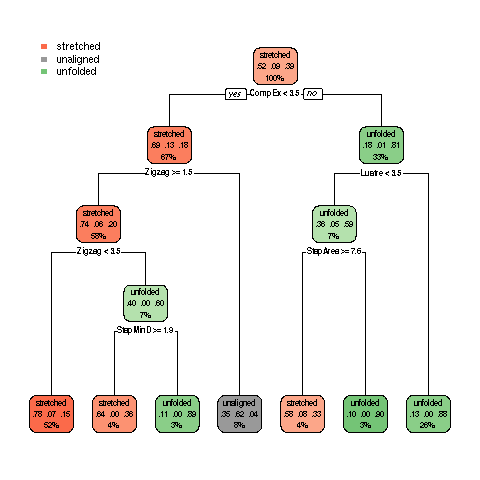
\includegraphics[width=1.1\textwidth]{figrpart1.png}
  \caption{Binary tree produced by recursive partitioning of 306 sheep data points using all 10 on-sheep scores and measures}
  \label{fig:rpart1}
\end{figure}

%\end{document}


We see the same partitioning as above. The percentages indicate the proportion of the data that has ended up in each node. There are 13 nodes.  It uses 6 of the 10 scores and measures. We end up with 60 percent stretched, 8 percent unaligned, and 32 percent unfolded.

	It is  possible to get a rating of the importance of each of the 10 scores and measures in constructing this partitioning. This is given below
\begin{verbatim}
Variable importance
   CompEx    Zigzag  StapArea  StapMaxD PeelScore  StapMinD    Lustre  Softness 
       38        19         9         9         8         6         5         4 
CrimpFreq 
        1 
\end{verbatim}
  Naturally, the traits it actually used come at the top of the list, but PeelScore rated quite highly and was not used. Whiteness did not rate at all, meaning that its importance was seen as zero.

	The only way we have available to judge the success of this classification tree is to use the recursive partitioning scheme of Figure~\ref{fig:rpart1} to classify the same learning data that were used to construct it.  That is not quite statistically valid, but there are no other data so we do it.  What we have to do is use the recursive partitioning tree to calculate a probability that each data item belongs to each CrimpType class. We get something like the following.

\begin{verbatim}
    stretched  unaligned   unfolded
1   0.1250000 0.00000000 0.87500000
2   0.1250000 0.00000000 0.87500000
3   0.7784810 0.06962025 0.15189873
4   0.7784810 0.06962025 0.15189873
5   0.7784810 0.06962025 0.15189873
.......
304 0.7784810 0.06962025 0.15189873
305 0.7784810 0.06962025 0.15189873
306 0.3461538 0.61538462 0.03846154
\end{verbatim}
  We then take the class with the highest probability as THE predicted class for each data item. So we get

\begin{verbatim}
> rpred(prpart1)
  [1] "unfolded"  "unfolded"  "stretched" "stretched" "stretched" "stretched"
  [7] "unfolded"  "stretched" "stretched" "stretched" "unaligned" "unfolded" 
.......
[295] "stretched" "unfolded"  "unfolded"  "unfolded"  "unfolded"  "stretched"
[301] "stretched" "stretched" "stretched" "stretched" "stretched" "unaligned"
\end{verbatim}
So one can see that the first sheep has been classified as "unfolded" because the probability is 0.875, and so on.

We can now construct a table ( commonly termed a 'confusion matrix') with rows showing prediced class, and columns showing actual class.
\begin{verbatim}
           actual
predicted   stretched unaligned unfolded
  stretched       137        12       32
  unaligned         9        16        1
  unfolded         12         0       87
\end{verbatim}
 So we have 137 correctly classed as 'stretched', 16 correctly classed as 'unaligned', and 87 correctly classed as 'unfolded'. This assumes that the actual CrimpType values are all correct - ie that our technique for looking at twist in fibre monts is perfect. It also violates some statistical niceties, which was mentioned above. But at least we have a success rate $240/306=0.78$. 

We should go on and identify the misclassified sheep, and try to see if they are just borderline cases on probability, or if they have some peculiarities. But there is something else which should be looked at first, and that is whether the tree in Figure~\ref{fig:rpart1} is overly elaborate. That is - did we use too many of the scores and measures and make too many nodes? 

The partitioning algorithm produces a number caller 'complexity parameter' to help control the depth of partitioning to an optimal level.  The CP measures the amount by which splitting a node improves the relative error. Here is the 'complexity parameter' table for the partitioning in Figure~\ref{fig:rpart1}.
\begin{verbatim}
> summary(rpart1)
Call:
rpart(formula = form.all, data = jan20sf2.df)
  n= 306 

          CP nsplit rel error    xerror       xstd
1 0.43918919      0 1.0000000 1.0000000 0.05906592
2 0.04729730      1 0.5608108 0.5608108 0.05254956
3 0.02702703      2 0.5135135 0.5945946 0.05349918
4 0.02027027      3 0.4864865 0.5945946 0.05349918
5 0.01013514      4 0.4662162 0.6013514 0.05367876
6 0.01000000      6 0.4459459 0.6148649 0.05402783
\end{verbatim}
 The column headed CP is the 'complexity parameter'. We see 6 splits ( 6 traits used) and a slow decline in complexity after the first split. The relative error ( called xerror in the above table ), has a minimum at just one split. It seems a bit drastic to stop at node 1.  We might, for example decide that the last 2 splits  are excessive. The way to deal with this is to do an operation called 'pruning' the tree. We use the complexity parameter to control the severity of 'pruning', so we will set it to $0.02$, as follows
\begin{verbatim}
rpart1.pruned <- prune(rpart1,cp=.02)
rpart1.pruned
n= 306 

node), split, n, loss, yval, (yprob)
      * denotes terminal node

 1) root 306 148 stretched (0.516339869 0.091503268 0.392156863)  
   2) CompEx< 3.5 204  64 stretched (0.686274510 0.132352941 0.181372549)  
     4) Zigzag>=1.5 178  47 stretched (0.735955056 0.061797753 0.202247191)  
       8) Zigzag< 3.5 158  35 stretched (0.778481013 0.069620253 0.151898734) *
       9) Zigzag>=3.5 20   8 unfolded (0.400000000 0.000000000 0.600000000)  
        18) StapMinD>=1.85 11   4 stretched (0.636363636 0.000000000 0.363636364) *
        19) StapMinD< 1.85 9   1 unfolded (0.111111111 0.000000000 0.888888889) *
     5) Zigzag< 1.5 26  10 unaligned (0.346153846 0.615384615 0.038461538) *
   3) CompEx>=3.5 102  19 unfolded (0.176470588 0.009803922 0.813725490) *
\end{verbatim}
So there are now only 9 nodes, and if we plot this 'pruned tree' we get the result shown in Figure~\ref{fig:rpart1p}
%\documentclass{article}
%\usepackage{graphicx,subfigure}
%\begin{document}

\begin{figure}[!h]
  \centering
  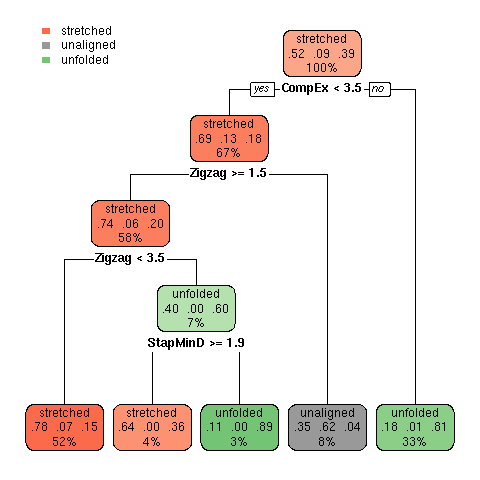
\includegraphics[width=1.1\textwidth]{figrpart1p.png}
  \caption{A pruned binary tree produced by removing the two least significant splits from Figure~\ref{fig:rpart1}}
  \label{fig:rpart1p}
\end{figure}

%\end{document}


which is considerably simplified. 

We can now use this pruned tree to classify the data, and we get the following confusion matrix
\begin{verbatim}
           actual
predicted   stretched unaligned unfolded
  stretched       130        11       28
  unaligned         9        16        1
  unfolded         19         1       91
\end{verbatim}
So we now have $237/306 = 0.77$ correctly classified. Not very different form the full tree.

We need to look a bit further, and see if we still have an 'ovefit' in terms of too many splits. So now we do another prune with the CP set to $0.03$, and we get
\begin{verbatim}
> rpart1.cp.03 <- prune(rpart1,cp=.03)
> rpart1.cp.03
n= 306 

node), split, n, loss, yval, (yprob)
      * denotes terminal node

1) root 306 148 stretched (0.516339869 0.091503268 0.392156863)  
  2) CompEx< 3.5 204  64 stretched (0.686274510 0.132352941 0.181372549)  
    4) Zigzag>=1.5 178  47 stretched (0.735955056 0.061797753 0.202247191) *
    5) Zigzag< 1.5 26  10 unaligned (0.346153846 0.615384615 0.038461538) *
  3) CompEx>=3.5 102  19 unfolded (0.176470588 0.009803922 0.813725490) *
> 
\end{verbatim}
 So there are now only 5 nodes , and the plot of this pruned tree is shown in Figure~\ref{fig:rpart1p2}
%\documentclass{article}
%\usepackage{graphicx,subfigure}
%\begin{document}

\begin{figure}[!h]
  \centering
  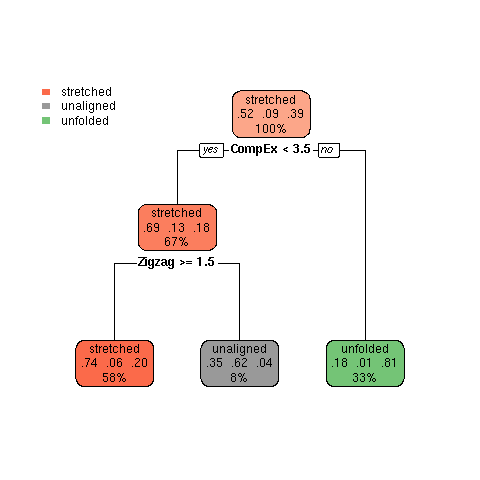
\includegraphics[width=1.1\textwidth]{figrpart1p2.png}
  \caption{A pruned binary tree produced by removing splits with a complexity parameter less than $0.03$ from Figure~\ref{fig:rpart1}}
  \label{fig:rpart1p2}
\end{figure}

%\end{document}


That is about as simplified as we can get. To separate 3 CrimpTypes we need a minimum of 2 splits.

If we now use this  very simple 2-split-tree to classify the data, we get the following confusion matrix
\begin{verbatim}
           actual
predicted   stretched unaligned unfolded
  stretched       131        11       36
  unaligned         9        16        1
  unfolded         18         1       83
\end{verbatim}
So we now have $230/306=0.75$ correctly classified. We are missing out on some of the unfolded cases. Perhaps we need that third split on $Zigzag < 3.5$.

So lets back off a bit and prune with $CP=0.025$. Then we get
\begin{verbatim}
> rpart1.cp.025 <- prune(rpart1,cp=.025)
> rpart1.cp.025
n= 306 

node), split, n, loss, yval, (yprob)
      * denotes terminal node

1) root 306 148 stretched (0.516339869 0.091503268 0.392156863)  
  2) CompEx< 3.5 204  64 stretched (0.686274510 0.132352941 0.181372549)  
    4) Zigzag>=1.5 178  47 stretched (0.735955056 0.061797753 0.202247191)  
      8) Zigzag< 3.5 158  35 stretched (0.778481013 0.069620253 0.151898734) *
      9) Zigzag>=3.5 20   8 unfolded (0.400000000 0.000000000 0.600000000) *
    5) Zigzag< 1.5 26  10 unaligned (0.346153846 0.615384615 0.038461538) *
  3) CompEx>=3.5 102  19 unfolded (0.176470588 0.009803922 0.813725490) *
> 
\end{verbatim}

So there are now 7 nodes. If we plot this pruned tree we get the result shown in Figure~\ref{fig:rpart1p25}
%\documentclass{article}
%\usepackage{graphicx,subfigure}
%\begin{document}

\begin{figure}[!h]
  \centering
  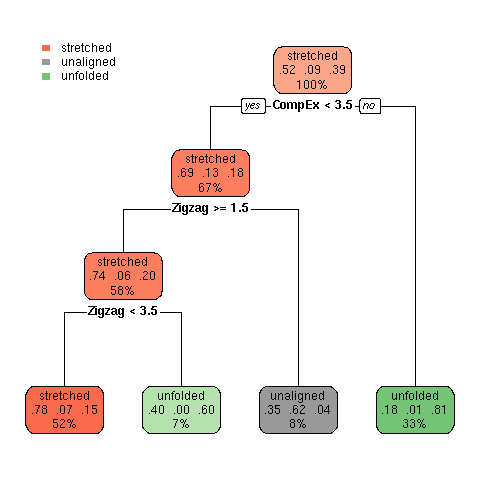
\includegraphics[width=1.1\textwidth]{figrpart1p25.png}
  \caption{A pruned binary tree produced by removing splits with a complexity parameter less than $0.025$ from Figure~\ref{fig:rpart1}}
  \label{fig:rpart1p25}
\end{figure}

%\end{document}



It uses Zigzag twice, once to split off the unaligned sheep, then again to split off a second batch of unfolded sheep.
If we use this 3 split tree to classify the data we get the following confusion matrix
\begin{verbatim}
           actual
predicted   stretched unaligned unfolded
  stretched       123        11       24
  unaligned         9        16        1
  unfolded         26         1       95
\end{verbatim}
So we now have $234/306=0.76$ correctly classified. There are less errors with the unfolded class , but more errors with the stretched class.  This is probably the best achievable result.

What we can now do is have a closer look at the misclassified animals. If we take the 24 animals predicted as stretched when the actual class was unfolded, and look at the probabilities for each class, we get
\begin{verbatim}
> str.unf.025 <- modsf2.df[paste(modsf2.df$pred.rpart1.cp.025,ct306,sep=":") == "stretched:unfolded",]
> prpart1.cp.025[as.integer(rownames(str.unf.025)),]
    stretched  unaligned  unfolded
26   0.778481 0.06962025 0.1518987
41   0.778481 0.06962025 0.1518987
47   0.778481 0.06962025 0.1518987
48   0.778481 0.06962025 0.1518987
.....
all 24 the same
\end{verbatim}
So all 24 are the same and these are not borderline cases, the is fairly certain, with Pr=0.77, that they are stretched.

If we now look at the opposite case, the 26 animalys classed as unfolded when the actual class was stretched. In this case the probabilities are
\begin{verbatim}
> unf.str.025 <- modsf2.df[paste(modsf2.df$pred.rpart1.cp.025,ct306,sep=":") == "unfolded:stretched",]
> prpart1.cp.025[as.integer(rownames(unf.str.025)),]
    stretched   unaligned  unfolded
42  0.4000000 0.000000000 0.6000000
43  0.4000000 0.000000000 0.6000000
62  0.4000000 0.000000000 0.6000000
64  0.1764706 0.009803922 0.8137255
69  0.1764706 0.009803922 0.8137255
71  0.1764706 0.009803922 0.8137255
86  0.1764706 0.009803922 0.8137255
118 0.1764706 0.009803922 0.8137255
131 0.1764706 0.009803922 0.8137255
138 0.4000000 0.000000000 0.6000000
141 0.1764706 0.009803922 0.8137255
144 0.1764706 0.009803922 0.8137255
151 0.1764706 0.009803922 0.8137255
153 0.1764706 0.009803922 0.8137255
154 0.4000000 0.000000000 0.6000000
169 0.1764706 0.009803922 0.8137255
186 0.1764706 0.009803922 0.8137255
191 0.1764706 0.009803922 0.8137255
209 0.4000000 0.000000000 0.6000000
210 0.4000000 0.000000000 0.6000000
232 0.1764706 0.009803922 0.8137255
234 0.1764706 0.009803922 0.8137255
250 0.4000000 0.000000000 0.6000000
280 0.1764706 0.009803922 0.8137255
294 0.1764706 0.009803922 0.8137255
296 0.1764706 0.009803922 0.8137255
> 
  these 26 differ   8 are .4, .6    rest are .17, .81
\end{verbatim}
So here it is different - there are 8 borderline cases ( with Pr=0.6 ), and 18 definite cases ( with Pr=0.8 ). 

The other thing we can do is compute the means for all measured traits for all nine groups in the above confusion table. This is given in Table~\ref{tab:misc025means}. We only get six of the nine cells from the confusion table because missing data for some of the traits has made the other 3 classes empty. We do have the most important cells.

% latex table generated in R 3.2.4 by xtable 1.8-2 package
% Mon Feb 13 20:58:10 2017
\begin{landscape}
\begin{table}[ht]
\centering
\caption{Means of all traits for animals in 6 of the 9 cells of the confusion matrix for a tree classification with complexity parameter 0.025}
\label{tab:misc025means}
\begin{tabular}{rllllll}
  \hline
 & 1 & 2 & 3 & 4 & 5 & 6 \\ 
  \hline
Trait & stretched:stretched & stretched:unfolded & unaligned:stretched & unaligned:unaligned & unfolded:stretched & unfolded:unfolded \\ 
  StapMaxD & 4.144 & 3.871 & 5.100 & 4.667 & 3.750 & 3.709 \\ 
  StapMinD & 2.237 & 2.014 & 2.500 & 2.300 & 1.900 & 1.891 \\ 
  StapArea &  9.463 &  7.914 & 11.700 & 10.633 &  7.250 &  7.170 \\ 
  CompEx & 2.781 & 3.000 & 2.000 & 2.000 & 3.500 & 3.913 \\ 
  Softness & 3.688 & 4.000 & 3.000 & 3.000 & 4.250 & 4.174 \\ 
  Lustre & 3.594 & 3.714 & 2.000 & 2.667 & 3.750 & 3.913 \\ 
  Whiteness & 3.406 & 3.714 & 3.000 & 3.667 & 4.000 & 3.565 \\ 
  PeelScore & 3.750 & 4.571 & 3.000 & 2.333 & 4.250 & 4.348 \\ 
  CrimpFreq & 3.456 & 3.614 & 4.000 & 3.633 & 3.375 & 3.691 \\ 
  Zigzag & 2.750 & 2.857 & 1.000 & 1.000 & 3.500 & 3.739 \\ 
  Dp & 16.356 & 14.957 & 14.100 & 13.367 & 16.025 & 15.222 \\ 
  SDDp & 2.675 & 2.514 & 2.700 & 2.333 & 3.050 & 2.639 \\ 
  Ds & 19.522 & 19.500 & 17.500 & 18.033 & 20.300 & 18.500 \\ 
  SDDs & 2.331 & 2.314 & 2.100 & 2.033 & 2.800 & 2.048 \\ 
  SovP & 25.025 & 23.700 & 31.200 & 24.467 & 23.925 & 26.243 \\ 
  Fn & 66.681 & 66.257 & 65.500 & 53.133 & 74.000 & 72.574 \\ 
  Dskin & 19.422 & 19.286 & 17.300 & 17.800 & 20.075 & 18.783 \\ 
  Bwt & 78.797 & 81.643 & 79.500 & 82.833 & 69.875 & 74.065 \\ 
  IGNorth & 122.562 & 166.857 & 128.000 &  66.667 &  74.000 & 182.174 \\ 
  IGSouth & 117.469 & 155.714 & 240.000 &  99.333 &  94.000 & 154.217 \\ 
  IGEast & 89.375 & 62.000 & 46.000 & 84.667 & 85.000 & 70.565 \\ 
  IGWest & 93.906 & 47.429 & 42.000 & 74.667 & 75.000 & 60.217 \\ 
  FollGpArea & 0.991 & 1.093 & 0.998 & 1.056 & 0.980 & 0.999 \\ 
  AreaPerFoll & 14051.75 & 13378.29 & 11885.00 & 15393.00 & 14155.25 & 12902.17 \\ 
  FollCurv & 1.938 & 2.000 & 3.000 & 2.333 & 2.250 & 2.130 \\ 
   \hline
\end{tabular}
\end{table}
\end{landscape}

The things that stand out are the IGNorth and IGSouth values for the "stretched:unfolded" class. They are huge. These sheep are obviously unfolded. The problem is that their CompEx and Zigzag scores are marginal, and the other scores and measurements do not seem to contribute much to sorting it out.

The "unfolded:stretched" class is the opposite. Their IGNorth and IGSouth values are tiny. These sheep are obviously stretched or unaligned. They are mistakenly assigned to unfolded because their CompEx and Zigzag scores are too high. Their staples are thin, like an unfolded sheep.  

The "unaligned:stretched" class is probably too small for the data to mean much. The staples are thick, like unaligned, and the CompEx and Zigzag scores are very small, again like unaligned, but the IGNorth and IGSouth values are large, like stretched. Mixed signals like that will cause confusion.

There is no obvious practical way to overcome these misclassifications at this stage.

\subsection{Linear discriminant functions}
We now look at finding functions of the ten on-sheep scores and measures which best discriminate between the three crimp types. This is different from principal components which simply finds functions with the largest variance. Linear discriminant functions maximize the ratio of between-crimp-class variance to within-crimp-class variance.

Again we use all the data, and ignore factors such as Flock, Age, and Sex. If we use all 10 on-sheep traits, the output from the {\em lda()} function is as follows
\begin{verbatim}
Call:
lda(form.all, data = jan20sf2.df)

Prior probabilities of groups:
 stretched  unaligned   unfolded 
0.51712329 0.09246575 0.39041096 

Group means:
          StapMaxD StapMinD  StapArea   CompEx Softness   Lustre Whiteness
stretched 4.585430 2.243709 10.720530 2.880795 3.496689 3.370861  3.324503
unaligned 6.618519 2.966667 20.937037 1.814815 2.185185 2.222222  3.185185
unfolded  3.711404 1.838596  7.138596 3.789474 3.982456 3.745614  3.543860
          PeelScore CrimpFreq   Zigzag
stretched  3.629139  3.723841 2.602649
unaligned  2.481481  4.596296 1.444444
unfolded   4.350877  4.006140 3.324561

Coefficients of linear discriminants:
                  LD1        LD2
StapMaxD  -0.23134246  0.7398803
StapMinD  -0.25068611  2.0371034
StapArea   0.01216284 -0.4175618
CompEx     0.76711265 -0.5745747
Softness   0.15307648  0.4626616
Lustre    -0.04925312  0.1563884
Whiteness -0.12597318 -0.5161429
PeelScore  0.28329899 -0.1031998
CrimpFreq  0.08761353 -0.3917679
Zigzag     0.56186076 -0.2722281

Proportion of trace:
   LD1    LD2 
0.8757 0.1243 
\end{verbatim}

The first thing we notice is that there are two discriminant functions ( labeled LD1 and LD2 )  in the above output, and that they explain 0.875 and 0.124 respectively of the between CrimpType variation. LD1 has heavy weights on CompEx and Zigzag, LD2 is dominated by StapMinD.

The next thing to notice is that all 10 traits have differences in their means for the stretched, unaligned, and unfolded groups. It is difficult to see, looking at the means, which traits should be used to discriminate. That is because the ten traits are correlated in a tangled fashion. The discriminant functions hopefully sort this out.

We again judge the success of these discriminant functions, by using them to classify the same learning data that were used to constuct them. We again make the warning that this is not quite statistically valid, and is likely to give an over-optimistic assessment of their success. We now use LD1 and LD2 to calculate the probability that each data item belongs to each CrimpType class. We get the following
\begin{verbatim}
$posterior
       stretched    unaligned     unfolded
1   2.122614e-01 4.353425e-06 7.877342e-01
2   3.155901e-02 7.297090e-07 9.684403e-01
3   7.616120e-01 7.817300e-04 2.376063e-01
4   8.315275e-01 1.417803e-03 1.670547e-01
5   9.423844e-01 1.518542e-03 5.609704e-02
6   8.351844e-01 5.483086e-04 1.642673e-01
........
304 8.894615e-01 1.255954e-02 9.797894e-02
305 8.515002e-01 4.850734e-04 1.480147e-01
306 8.515308e-01 1.431656e-01 5.303645e-03
\end{verbatim}
As before, we take the class with the highest probability as THE predicted class for each data item. So we get
\begin{verbatim}
$class
  [1] unfolded  unfolded  stretched stretched stretched stretched unfolded 
  [8] stretched stretched stretched stretched unfolded  unfolded  <NA>     
........
[295] stretched unfolded  unfolded  <NA>      unfolded  <NA>      unfolded 
[302] stretched stretched stretched stretched stretched
\end{verbatim}
 So one can see that the first sheep has been classified as "unfolded" because the probability is 0.788, and so on. We should note that there are NA's; in R NA means 'not available' and comes from sheep with missing data. The previous recursive partitioning procedure assigned such sheep the prior probabilities for each CrimpType. Prior probabilities are simply the frequency of each group in the data. The present discriminant function procedure does not attempt to classify such sheep. So we have to be careful comparing confusion tables, because the linear discriminant function confusion tables will not have 306 sheep in total.

So if we now construct the confusion table for the present case we get
\begin{verbatim}
           actual
predicted   stretched unaligned unfolded
  stretched       123        11       19
  unaligned         7        16        1
  unfolded         21         0       94
\end{verbatim}
So we have 123 correctly classed as 'stretched', 16 correctly classed as 'unaligned', and 94 correctly classed as 'unfolded'. We have a success rate of $233/292= 0.79$ with 14 sheep left unclassified. This is almost exactly the same as for recursive partitioning with all 10 traits.

We are using 2 discriminant functions. We need to discriminate in 2 dimensions because there are 3 CrimpType classes to separate. We can look at how well the 3 CrimpType classes separate in these 2 dimensions by plotting the values of the LD1 and LD2 functions for all the sheep. This is shown in Figure~\ref{fig:lda1}
%\documentclass{article}
%\usepackage{graphicx,subfigure}
%\begin{document}

\begin{figure}[!h]
  \centering
  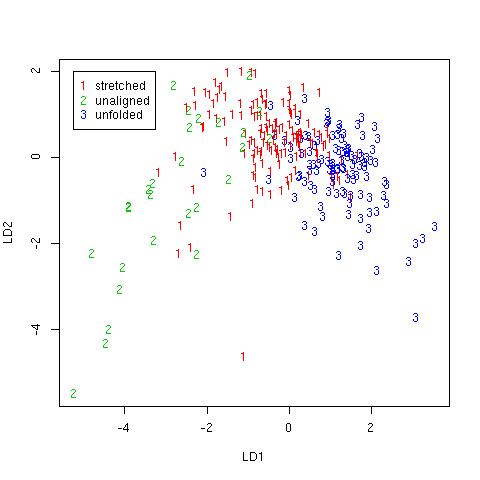
\includegraphics[width=1.1\textwidth]{figlda1.png}
  \caption{Plot of the two discriminant function values for the case with all 10 traits included showing how the CrimpType groups separate}
  \label{fig:lda1}
\end{figure}

%\end{document}


We can see that LD1 separates the 3 CrimpTypes in order $unaligned < stretched < unfolded$, but there is not a complete separation. LD2 tends to have high values for stretched and lower values for the other two types.

There is no equivalent, for discriminant functions, of the procedure used to 'prune' a classification tree. We can decide that a trait is not contributing and drop it from the discriminant function, but the analysis just about does that for you anyway. In the present case, it would seem that all traits are of some importance because they all have sizeable coefficients in one or both of the discriminant functions LD1 and LD2.

So we are just going to try dropping CrimpFreq because there are intuitive reasons for thinking that it has nothing to do with CrimpType. We get a 9 trait analysis as follows
\begin{verbatim}
Call:
lda(form.2, data = jan20sf2.df)

Prior probabilities of groups:
 stretched  unaligned   unfolded 
0.51677852 0.09060403 0.39261745 

Group means:
          StapMaxD StapMinD  StapArea   CompEx Softness   Lustre Whiteness
stretched 4.573377 2.246104 10.719481 2.876623 3.506494 3.376623  3.324675
unaligned 6.618519 2.966667 20.937037 1.814815 2.185185 2.222222  3.185185
unfolded  3.714530 1.837607  7.138462 3.777778 3.982906 3.752137  3.547009
          PeelScore   Zigzag
stretched  3.629870 2.610390
unaligned  2.481481 1.444444
unfolded   4.350427 3.316239

Coefficients of linear discriminants:
                  LD1        LD2
StapMaxD  -0.20627716  0.8397969
StapMinD  -0.29378638  2.5699488
StapArea   0.00925765 -0.4791005
CompEx     0.75458869 -0.6435115
Softness   0.15634672  0.5184283
Lustre    -0.06600363  0.3585171
Whiteness -0.11671974 -0.6438872
PeelScore  0.31168152 -0.2161910
Zigzag     0.53505528 -0.1685627

Proportion of trace:
   LD1    LD2 
0.8881 0.1119 
\end{verbatim}

This is virtually identical with the 10 trait case, except that CrimpFreq is not there. If we go ahead and do the prediction using all data and construct the confusion table we get
\begin{verbatim}
           actual
predicted   stretched unaligned unfolded
  stretched       126        11       18
  unaligned         5        16        1
  unfolded         23         0       98
\end{verbatim}
So we have a success rate of $240/298 = 0.805 $ which is just slightly better than the 10 trait case. So CrimpFreq is probably just contributing noise.

The plot of LD1 versus LD2 for all sheep in the 9 trait case is shown in Figure~\ref{fig:lda2}.
%\documentclass{article}
%\usepackage{graphicx,subfigure}
%\begin{document}

\begin{figure}[!h]
  \centering
  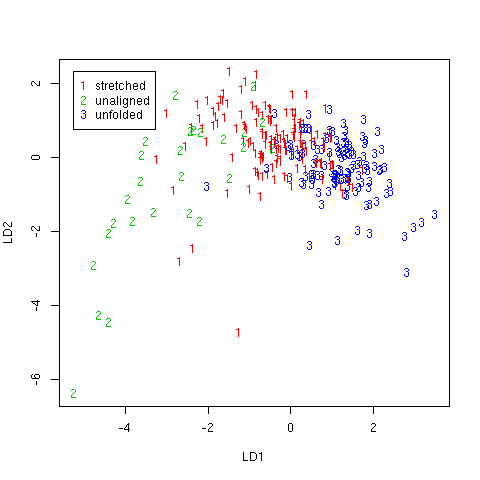
\includegraphics[width=1.1\textwidth]{figlda2.png}
  \caption{Plot of the two discriminant function values for the case with 9 traits included showing how the CrimpType groups separate}
  \label{fig:lda2}
\end{figure}

%\end{document}


The separation in this plot is almost the same as in the 10 trait plot. 

So from the superior confusion matrix and the almost identical plot we conclude that the 9 trait case omitting CrimpFreq is acceptable.

On the same 'we think' basis, we might try dropping StapArea, because it is just a function of StapMaxD and StapMinD and is therefore likely to be redundant. So we now do an 8 trait analysid which gives
\begin{verbatim}
Call:
lda(form.8, data = jan20sf2.df)

Prior probabilities of groups:
stretched unaligned  unfolded 
0.5183946 0.0903010 0.3913043 

Group means:
          StapMaxD StapMinD   CompEx Softness   Lustre Whiteness PeelScore
stretched 4.564516 2.241290 2.877419 3.509677 3.380645  3.329032  3.638710
unaligned 6.618519 2.966667 1.814815 2.185185 2.222222  3.185185  2.481481
unfolded  3.714530 1.837607 3.777778 3.982906 3.752137  3.547009  4.350427
            Zigzag
stretched 2.612903
unaligned 1.444444
unfolded  3.316239

Coefficients of linear discriminants:
                  LD1        LD2
StapMaxD  -0.18570146 -0.3907957
StapMinD  -0.24207299  0.3504842
CompEx     0.76181766 -0.9206114
Softness   0.16458848  0.7034348
Lustre    -0.07123684  0.7753099
Whiteness -0.12466371 -0.8554602
PeelScore  0.29958827 -0.2303394
Zigzag     0.53439568 -0.1468362

Proportion of trace:
   LD1    LD2 
0.9419 0.0581 
\end{verbatim}
So here, LD1 has similar coefficients for the traits still there, but LD2 is alittle different. If we go ahead and do the prediction using all data and construct the confusion table we get
\begin{verbatim}
           actual
predicted   stretched unaligned unfolded
  stretched       125        11       20
  unaligned         7        16        2
  unfolded         23         0       95
\end{verbatim}
 So we now get $236/299 = 0.789$ which is back to what we had with the 10 trait case, and a little worse than the 9 trait case.

The plot of LD1 versus LD2 for all sheep for the 8 trait case is shown in Figure~\ref{fig:lda8}
%\documentclass{article}
%\usepackage{graphicx,subfigure}
%\begin{document}

\begin{figure}[!h]
  \centering
  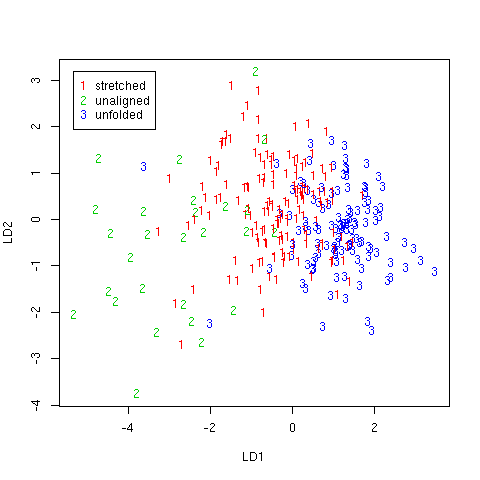
\includegraphics[width=1.1\textwidth]{figlda8.png}
  \caption{Plot of the two discriminant function values for the case with 8 traits included showing how the CrimpType groups separate}
  \label{fig:lda8}
\end{figure}

%\end{document}


In this case, LDA2 seems to contribute very little to separation. We should stay with the previous 9 trait case. We have lost something by omitting StapArea, particularly with separating the unaligned group. Perhaps StapArea, being an average, is more accurate than either StapMaxD or StapMinD.

There remains the  question of what are the misclassified animals in the discriminant function case. We first check to see if they are the same animals as those misclassified by recursive partitioning. The table below copmares the classification of the pruned tree with $CP=0.025$ ( considered to be the best tree classification) with the classification by a linear discriminant function with 9 traits ( considered to be the best discriminant function classification).
\begin{verbatim}
           lda
rpart       stretched unaligned unfolded
  stretched       137         4       10
  unaligned         8        18        0
  unfolded         10         0      111
\end{verbatim}
 So they are not the same, or all the off-diagonal counts would be zero.

That means we have to look separately at what are the animals misclassified by the discriminant function. We look first at the 18 animals classed as stretched when the actual class was unfolded, and look at the probabilities for each class we get.
\begin{verbatim}
> str.unf.d2  <- modsf2.df[paste(modsf2.df$pred.d2,ct306,sep=":") == "stretched:unfolded",]
> pd2$posterior[as.integer(rownames(str.unf.d2)),]
    stretched    unaligned   unfolded
26  0.9035270 1.470277e-03 0.09500268
41  0.6931238 2.994676e-04 0.30657670
47  0.7435326 1.258013e-03 0.25520937
49  0.8298894 3.252161e-03 0.16685847
50  0.4985387 4.867091e-01 0.01475218
53  0.6487102 1.014571e-03 0.35027526
55  0.6644680 2.362903e-04 0.33529574
98  0.6232317 3.199086e-03 0.37356919
100 0.6253530 9.031581e-04 0.37374387
116 0.6437613 5.048662e-04 0.35573385
148 0.5618719 3.138781e-05 0.43809667
149 0.7556986 1.562294e-03 0.24273907
195 0.7154989 3.713676e-04 0.28412971
196 0.5525998 2.562927e-04 0.44714390
197 0.7159998 1.573846e-04 0.28384282
219 0.8142730 1.236185e-02 0.17336511
224 0.7026830 1.634226e-03 0.29568280
272 0.6102583 6.610055e-04 0.38908069
> 
\end{verbatim}
The probabilities for stretched are high ( greater than 0.7) for 8 animals, there are 7 with probabilities 0.6 to 0.7, and 3 below 0.6. So there are quite a few borderline cases, all except one being  borderline with unfolded. 

If we now look at the opposite case, the 23 animals classed as unfolded when the actual class was stretched, we find the following probabilities
\begin{verbatim}
> unf.str.d2 <- modsf2.df[paste(modsf2.df$pred.d2,ct306,sep=":") == "unfolded:stretched",]
> pd2$posterior[as.integer(rownames(unf.str.d2)),]
    stretched    unaligned  unfolded
42  0.4709088 1.045100e-04 0.5289867
62  0.3926636 2.106521e-04 0.6071257
69  0.2013635 9.363961e-05 0.7985428
86  0.1143817 2.036105e-05 0.8855979
118 0.1067955 6.184228e-06 0.8931983
131 0.3516904 8.901992e-05 0.6482206
138 0.4539394 5.090208e-05 0.5460097
141 0.3038035 1.025338e-04 0.6960939
151 0.1689961 5.743036e-05 0.8309465
153 0.2984161 8.338542e-05 0.7015005
154 0.3997118 2.022290e-04 0.6000860
169 0.1481053 2.721703e-05 0.8518674
186 0.4235852 5.681640e-05 0.5763579
191 0.1555985 2.885044e-05 0.8443726
198 0.4327509 1.097268e-04 0.5671394
200 0.3992365 2.181659e-04 0.6005453
228 0.3128537 2.473241e-04 0.6868990
232 0.4505216 7.190134e-04 0.5487593
234 0.1439119 5.604178e-05 0.8560320
250 0.4130386 4.883455e-05 0.5869126
280 0.4728361 7.769729e-05 0.5270862
294 0.4365274 2.898286e-04 0.5631828
296 0.2829702 7.565116e-05 0.7169541
> 
\end{verbatim}
The probabilities for unfolded are high for 9 animals, med for 6 animals, and low for 8 animals. So there are again a lot of borderline cases. All of the confusion is between stretched and unfolded.

If we now compute the means for all measurted traits for all nine groups in the confusion table for the discriminant function case with 9 traits, we get Table~\ref{tab:misclda9means}. Again we only get 6 of the 9 cells from the confusion table because of missing data for some traits. 

For the "stretched:unfolded" class ( classed as stretched when actual was unfolded) the IGNorth and IGSouth means are intermediate ( not huge like for the recursive tree case) and the CompEx and Zigzag scores are intermediate too. There is nothing unusual about these misclassified sheep.

For the "unfolded:stretched" case the IGNorth and IGSouth values are tiny. These sheep are clearly genuine stretched cases. The CompEx and Zigzag scores are greater than 3 on average, so the confusion probably comes from this. They also have a high Whiteness and Lustre mean score, and the staples are small. These are tricky sheep to class correctly, they break all the 'rules'.

% latex table generated in R 3.2.4 by xtable 1.8-2 package
% Fri Feb 17 21:10:42 2017
\begin{landscape}
\begin{table}[ht]
\centering
\caption{Means of all traits for animals in 6 of the 9 cells of the confusion matrix for a linear discriminant function classification with 9 traits ( all except CrimpFreq).}
\label{tab:misclda9means}
\begin{tabular}{rlllll}
  \hline
 & 1 & 2 & 3 & 4 & 5 \\ 
  \hline
Trait & stretched:stretched & stretched:unaligned & stretched:unfolded & unfolded:stretched & unfolded:unfolded \\ 
  StapMaxD & 4.226 & 4.667 & 4.483 & 3.617 & 3.562 \\ 
  StapMinD & 2.297 & 2.300 & 2.150 & 1.750 & 1.862 \\ 
  StapArea &  9.832 & 10.633 &  9.717 &  6.450 &  6.750 \\ 
  CompEx & 2.742 & 2.000 & 3.000 & 3.333 & 3.875 \\ 
  Softness & 3.645 & 3.000 & 4.333 & 4.167 & 4.083 \\ 
  Lustre & 3.516 & 2.667 & 3.833 & 3.833 & 3.875 \\ 
  Whiteness & 3.387 & 3.667 & 3.333 & 3.833 & 3.667 \\ 
  PeelScore & 3.645 & 2.333 & 4.167 & 4.500 & 4.458 \\ 
  CrimpFreq & 3.458 & 3.633 & 3.350 & 3.483 & 3.754 \\ 
  Zigzag & 2.677 & 1.000 & 3.167 & 3.333 & 3.625 \\ 
  Dp & 16.381 & 13.367 & 14.683 & 15.633 & 15.279 \\ 
  SDDp & 2.697 & 2.333 & 2.533 & 2.817 & 2.629 \\ 
  Ds & 19.474 & 18.033 & 19.233 & 19.950 & 18.608 \\ 
  SDDs & 2.332 & 2.033 & 2.233 & 2.600 & 2.079 \\ 
  SovP & 25.213 & 24.467 & 23.033 & 24.350 & 26.304 \\ 
  Fn & 65.816 & 53.133 & 61.733 & 75.833 & 73.442 \\ 
  Dskin & 19.377 & 17.800 & 19.033 & 19.733 & 18.867 \\ 
  Bwt & 79.387 & 82.833 & 72.583 & 69.917 & 76.646 \\ 
  IGNorth & 126.065 &  66.667 & 135.667 &  73.000 & 189.333 \\ 
  IGSouth & 124.290 &  99.333 & 115.667 &  87.000 & 164.292 \\ 
  IGEast & 86.516 & 84.667 & 60.000 & 94.000 & 70.708 \\ 
  IGWest & 90.806 & 74.667 & 40.833 & 88.667 & 61.333 \\ 
  FollGpArea & 0.993 & 1.056 & 1.035 & 0.975 & 1.017 \\ 
  AreaPerFoll & 14083.00 & 15393.00 & 13657.33 & 13598.17 & 12852.25 \\ 
  FollCurv & 1.968 & 2.333 & 1.667 & 2.167 & 2.208 \\ 
   \hline
\end{tabular}
\end{table}
\end{landscape}



\subsection{Discriminating 2 classes at a time}
A linear discriminator trying to separate 3 classes has to make compromises. We may be able to give the technique a bit more room to move in by attacking the problem 2 classes at a time. We first divided the data into (unfolded + stretched) versus unaligned and constructed a linear discriminant function for these 2 groups. The result is shown below
\begin{verbatim}
> unfstr.lda
Call:
lda(form.unfstr, data = modsf2.df)

Prior probabilities of groups:
    unfstr       unal 
0.90753425 0.09246575 

Group means:
       StapMaxD StapMinD  StapArea   CompEx Softness   Lustre Whiteness
unfstr 4.209434 2.069434  9.179623 3.271698 3.705660 3.532075  3.418868
unal   6.618519 2.966667 20.937037 1.814815 2.185185 2.222222  3.185185
       PeelScore CrimpFreq   Zigzag
unfstr  3.939623  3.845283 2.913208
unal    2.481481  4.596296 1.444444

Coefficients of linear discriminants:
                  LD1
StapMaxD  -0.18846462
StapMinD  -0.81385171
StapArea   0.19677221
CompEx    -0.30222705
Softness  -0.34520555
Lustre    -0.03956518
Whiteness  0.35090151
PeelScore -0.16540082
CrimpFreq  0.12642892
Zigzag    -0.29469897
\end{verbatim}
So we get just one function (LD1) which best separated unaligned from the rest.
This was relatively successful as shown in the fowllowing confusion table
\begin{verbatim}
> table(predicted=punfstr.lda$class,modsf2.df$ctunfstr)
         
predicted unfstr unal unfstr
   unfstr    257   11      0
   unal        8   16      0
   unfstr      0    0      0
\end{verbatim}
So we get $273/292=0.93$ correct classifications. That is a substantial improvement. It is, of course, an easier problem just to separate out the unaligned shep.

We then divided the data into (stretched + unaligned) versus unfolded, and constructed the following linear discriminator. 
\begin{verbatim}
> strunal.lda
Call:
lda(form.strunal, data = modsf2.df)

Prior probabilities of groups:
 strunal      unf 
0.609589 0.390411 

Group means:
        StapMaxD StapMinD  StapArea   CompEx Softness   Lustre Whiteness
strunal 4.893820 2.353371 12.270225 2.719101 3.297753 3.196629  3.303371
unf     3.711404 1.838596  7.138596 3.789474 3.982456 3.745614  3.543860
        PeelScore CrimpFreq   Zigzag
strunal  3.455056   3.85618 2.426966
unf      4.350877   4.00614 3.324561

Coefficients of linear discriminants:
                  LD1
StapMaxD  -0.50258124
StapMinD  -1.06739812
StapArea   0.18667019
CompEx     0.87142191
Softness  -0.07042477
Lustre    -0.10652068
Whiteness  0.11525528
PeelScore  0.27569564
CrimpFreq  0.23754866
Zigzag     0.57536961
\end{verbatim}
So again there is just one function (LD1), and it is also quite successful as shown in the following confusion table.
\begin{verbatim}
> table(predicted=pstrunal.lda$class,actual=modsf2.df$ctstrunal)
         actual
predicted strunal strunal unf
  strunal     156       0  22
  strunal       0       0   0
  unf          22       0  92
\end{verbatim}
So now we get $248/292=0.84$ successful classifications.
 Both cases were more successful than the pair of discriminant functions designed to best discriminate between 3 groups

We can compute the value of these 2 separate discriminant functions for each sheep, and plot them as if they were 2 observed traits as shown in Figure~\ref{fig:ldunal_ldunf}.
%\documentclass{article}
%\usepackage{graphicx,subfigure}
%\begin{document}

\begin{figure}[!h]
  \centering
  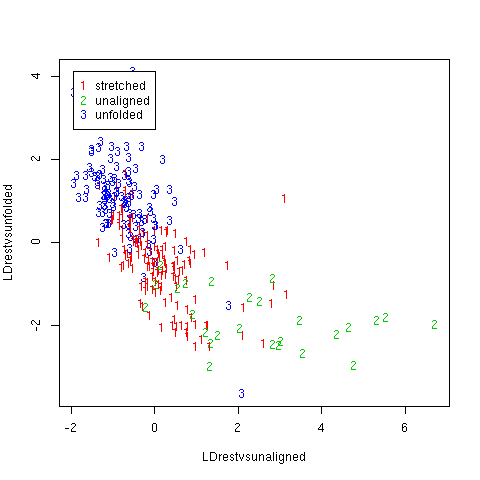
\includegraphics[width=1.1\textwidth]{figldunal_ldunf.png}
  \caption{Plot of the values of the discriminant function between unaligned and the rest, against values of the discriminant function between unfolded and the rest, for all 306 sheep, with the actual class of each sheep shown as colour coded digits as set out in the legend}
  \label{fig:ldunal_ldunf}
\end{figure}

%\end{document}



This seems to give better separation ( at least visually).

We need to try to interpret the two axes on Figure~\ref{fig:ldunal_ldunf}. The LDrestvsunaligned axis should represent what is different about unaligned wools, that is poor fibre alignment. So one would expect the linear function to have significant negative weights on PeelScore, Lustre, and Softness. Well it does have -0.34 on Softness, and it has -.81 on StapMinD, but it also uses Compex and Zigzag negatively. So it makes sense, but it is not only alignment, it is crimp appearance too.

The LDrestvsunfolded axis we would expect to represent what is different about unfolded wools, that is space between follicle groups in the skin. So one would expect significant weights on Whiteness and StapMinD(negative). Well it does have -1.06 on StapMinD, but only 0.11 on Whiteness, but is also uses CompEx and Zigzag ( positively), So again, it makes sense, but it is not only 'space', it is crimp appearance too. 

We can actually test the above ideas. Make up three indices of alignment , space, and crimp appearance as follows
\begin{eqnarray*}
align & = & PeelScore * Lustre * Softness \\
space & = & Whiteness / StapMinD \\
crimp & = & CompEx * Zigzag / CrimpFreq
\end{eqnarray*}
Then plot 'align' and 'space' identifying the CrimpType of each point as in  Figure~\ref{fig:ldunal_ldunf}, and we get Figure~\ref{fig:align_space}
%\documentclass{article}
%\usepackage{graphicx,subfigure}
%\begin{document}

\begin{figure}[!h]
  \centering
  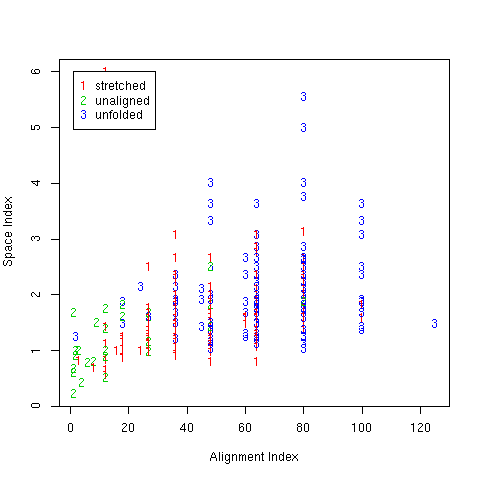
\includegraphics[width=1.1\textwidth]{figalign_space.png}
  \caption{Plot of the values of our aligment index , against values of our space index  for all 306 sheep, with the actual class of each sheep shown as colour coded digits as set out in the legend}
  \label{fig:align_space}
\end{figure}

%\end{document}


We see that there some separation of the 3 CrimpTypes based on alignment index and space index alone, but not as good a separation as in Figure~\ref{fig:ldunal_ldunf}. The pattern of points now has a positive slope because our alignment index is the reverse of the LDrestvsunaligned function. 

We also plot 'align' and 'crimp' in Figure~\ref{fig:align_crimp}, and 'space' and 'crimp' in Figure~\ref{fig:space_crimp}. The separation is similar in all three plots.
%\documentclass{article}
%\usepackage{graphicx,subfigure}
%\begin{document}

\begin{figure}[!h]
  \centering
  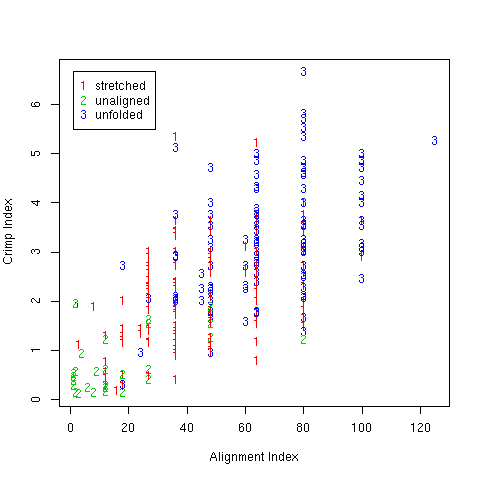
\includegraphics[width=1.1\textwidth]{figalign_crimp.png}
  \caption{Plot of the values of our aligment index , against values of our crimp index  for all 306 sheep, with the actual class of each sheep shown as colour coded digits as set out in the legend}
  \label{fig:align_crimp}
\end{figure}

%\end{document}


%\documentclass{article}
%\usepackage{graphicx,subfigure}
%\begin{document}

\begin{figure}[!h]
  \centering
  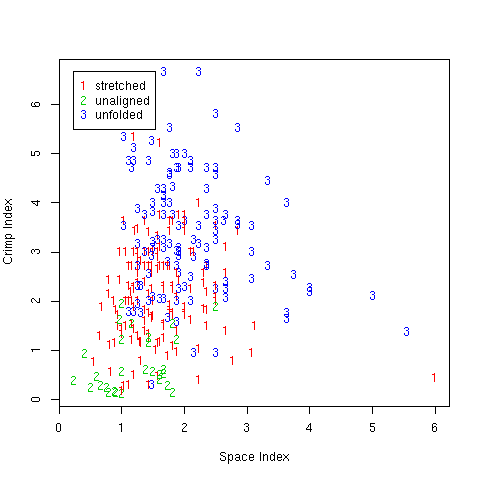
\includegraphics[width=1.1\textwidth]{figspace_crimp.png}
  \caption{Plot of the values of our space index , against values of our crimp index  for all 306 sheep, with the actual class of each sheep shown as colour coded digits as set out in the legend}
  \label{fig:space_crimp}
\end{figure}

%\end{document}



This helps confirm our interpretation of the two discriminant functions above.  It also suggests that we need the crimp appearance scores (CompEx and Zigzag)  as well as alignment and space, to achieve a reasonable separation of the three CrimpTypes. There is one animal of class stretched that has an outlier value of 5.9 for 'space' index. It has $StapMinD = 0.5$. That may be an error.


It is an option to apply these two linear discriminators sequentially. So we use the first function and put aside $8 + 16 = 24$ sheep identified as unaligned. Then we take the remaining  268 sheep and use the second function on those. We get
\begin{verbatim}
> table(predicted=pstrunal276.lda$class,actual=ct306[punfstr.lda$class != "unal"])
         actual
predicted stretched unaligned unfolded
  strunal       123        11       21
  strunal         0         0        0
  unf            21         0       92
\end{verbatim}
We now identify $92 + 21 = 113$ sheep as unfolded, and we have to presume that the remaining 155 are stretched.
So we end up with a two-step success rate of $231/292=.79$ , which is no better than using one discriminant function to separate 3 groups.

The two-step procedure makes sense - in terms of being able to interpret the disciminant functions - but it does not improve the overall outcome, which is surprising as each of the two steps separately has a better success rate, but when we put them together it drops back to the same as doing 3 groups in one hit.


\subsection{Flock differences}
We need to investigate whether a classifier developed on data from one ( or more) flocks works equally well when used on another new flock. This is difficult with the present data because the number of sheep per flock is small. Classifiers, especially discriminant functions, depend on covariance matrices and these need reasonable numbers of sheep for estimation.

What we can do is use flocks 1-6 to develop a discriminator, then apply it to flocks 7-12. So starting with flocks 1 to 6, we fit the following discriminator using 9 traits ( ie omitting CrimpFreq)
\begin{verbatim}
> d2.1to6
Call:
lda(form.2, data = sf2.1to6.df)

Prior probabilities of groups:
stretched unaligned  unfolded 
0.5000000 0.1287879 0.3712121 

Group means:
          StapMaxD StapMinD StapArea   CompEx Softness   Lustre Whiteness
stretched 4.781818 2.274242 11.42273 2.863636 3.363636 3.272727  3.181818
unaligned 7.447059 3.082353 23.91765 1.647059 1.588235 1.705882  3.058824
unfolded  3.689796 1.802041  6.95102 3.673469 3.897959 3.632653  3.469388
          PeelScore   Zigzag
stretched  3.575758 2.393939
unaligned  2.294118 1.294118
unfolded   4.285714 3.183673

Coefficients of linear discriminants:
                  LD1        LD2
StapMaxD  -0.48426165  0.6097882
StapMinD  -0.45091199  2.0106702
StapArea   0.05798470 -0.3365145
CompEx     0.72314833 -0.5550316
Softness   0.29955089  0.5325906
Lustre    -0.08011584  0.7550601
Whiteness -0.23801308 -0.7151770
PeelScore  0.13533827 -0.4405284
Zigzag     0.47786349 -0.5153478

Proportion of trace:
  LD1   LD2 
0.886 0.114 
\end{verbatim}
 These functions ( LD1 and LD2 above) have similar coefficients to those obtained using 9 traits on all 12 flocks. The proportions of variance explained are also similar.

 We now apply these functions, firstly to their own flock 1 to 6 data and get
\begin{verbatim}
> table(predicted=pd2.1to6$class,actual=sf2.1to6.df$CrimpType)
           actual
predicted   stretched unaligned unfolded
  stretched        55         3        9
  unaligned         3        14        0
  unfolded          8         0       40
> 
\end{verbatim}
This has a success rate of $109/132=0.82$, which is slightly better than on the full 12 flock data. 

We then apply these same functions to flocks 7 to 12 and get
\begin{verbatim}
> table(predicted=pd2.7to12$class,actual=sf2.7to12.df$CrimpType)
           actual
predicted   stretched unaligned unfolded
  stretched        63         9        8
  unaligned         1         1        1
  unfolded         24         0       59
> 
\end{verbatim}
This has a lower success rate of $123/165=0.74$. This is not a very serious amount of 'slippage' in moving to another data set. 

So the discriminant functions are robust.

\section{Discussion}
There is not a large difference between the recursive tree approach and the discriminant function approach to classification. The tree approach is limited to considering one trait only at each split, and it draws a cutoff line parallel to the axis for that trait. The discriminant function approach considers all traits at once and only does one split. It is capable of drawing cutoff lines at angles to the axes, and therefore is intrinsically 'better'. In practice there is  little difference between the two techniques.

We were able to put some sort of an interpretation on what the various classifiers are doing. From our knowledge of the factors which are important in forming crimp as outlined in Jackson and Watts(2016)~\cite{jack:16}, we were able to intuitively group the visual traits into factors which we called 'alignment', 'space', and 'crimp appearance'. We were able to show that the discriminant functions did something similar. So while the discriminant function analysis is not causal, it does tend to separate the causal factors (space and alignment), but it can not do it completely because there are only 2 discriminant functions, and there are 3 factors involved. The 'crimp appearance' factor tends to  dominate the tree splits, and tends to appear in all discriminant functions, somewhat masking the role of the causal 'align' and 'space' causal factors.

There is a technique called quadratic discriminant functions. We tried it on these data. It  is capable of drawing curved cutoff lines. It was slightly lesss effective than the linear discriminant functions. Results are not reported.

The biggest issue with the present data is that there simply is not a complete separation of the three CrimpTypes, no matter how much statistical manipulation we engage in. We either have to accept that the grading of sheep into three CrimpTypes is an attempt to put 3 classes on a continuum, or we have to search for some further visual observations which might help to better separate the classes. 

It is probably true that the unaligned grade shades into the stretched grade. We may have to live with that. It is the confusion between stretched and unfolded grades that surprises, given that we know that the mechanisms for forming stretched and unfolded crimp are entirely different, and that a given sheep can only be one or the other.

There are mistakes between stretched and unfolded in both directions. Some are what we call 'borderline' cases - the probabilities are close to a 50/50 bet between stretched and unfolded. Others are 'gross mistakes' - the classification procedure is quite sure( ie with a high probability) of its grade, but it is wrong.

We were able to check up on  the CrimpType grades, made by looking for 'twist' on fibre mounts, by looking at the skin data, particularly the IGNorth and IGSouth distances. The grades look to be OK. It is the visual data that are somehow not seeing everything.
 

\begin{thebibliography}{99}

\bibitem{brei:84}
Breiman L., Friedman J.H., Olshen R.A., and Stone C.J. (1984)
Classification and Regression Trees. Wadsworth, California, 1984


\bibitem{jack:16}
Jackson, N. and Watts, J.E. (2016) Staple crimp formation in the fleece of Merino sheep. Unpublished manuscript, 18 May 2016.

\bibitem{onio:62}
Onions, W.J. (1962) Wool: an introduction to its properties, varieties, uses
     and production. Ernest Benn limited, London, 1962

\bibitem{rprog:13}
R Core Team (2013). R: A language and environment for statistical
  computing. R Foundation for Statistical Computing, Vienna, Austria.
  ISBN 3-900051-07-0, URL http://www.R-project.org/.

\bibitem{vena:99}
Venables, W.N. and Ripley, B.D. (1999)
Modern Applied Statistics with S-Plus, 3rd Ed. Springer, New York

\end{thebibliography}
\end{document}
